\section{Mission analysis and \texorpdfstring{$\Delta V$}{Delta-V} budget}
\label{sec:ma_and_dv}

\subsection{Rationale of the mission analysis}
\label{subsec:rationale_ma}

The mission analysis previously described could be split into two macro-categories:
\begin{itemize}
    \item From launch to the interplanetary transfer, including DSMs and the Earth fly-by;
    \item Planetary phase around Jupiter.
\end{itemize}
The main objectives of the mission analysis were to keep the overall launch energy $C_3$ and determinstic $\Delta V$ as low as possible, compliant with the constraints imposed by the navigation and spacecraft operational requirements. Regarding the interplanetary transfer, two main options were available, both including an EGA. The first option, named as "$2- dV\,EGA$", contemplated a launch window timeframe in October-November 2011. However, the latter was discarded since the approach angle at Jupiter would have resulted in a latitude farther away from the equator. This would have brought to higher radiation levels, hence a reduced time available for the science operations \cite{launch_period}. The second option, named as "$2+  dV\,EGA$", contemplated a launch window timeframe in August 2011 and it ended up being the chosen one. A viable back-up of this transfer would have happened in October 2012, since the basic features of "$2+ dV\,EGA$" repeat every 13 months.
Regarding the interplanetary trajectory constraints, they could be divided into three categories:
\begin{itemize} 
    \item \textbf{Launch energy $C_3$ and timing constraints.} Fixing an inital value for the energy provided by the launcher, different possibilites of departure date could be analyzed. Every launch date defined a trajectory that was characterized by a required $C_3$ and determinstic $\Delta V$. The maximum $C_3 = 31.1 km^2 / s^2$ was defined by the Atlas V551 launcher \cite{atlasV_juno}. Analyzing Juno's ephemerides for the actual launch date, the calculated value is $C_3 = 31.08 km^2 / s^2$. The trajectory reconstructed through the optimization problem and explained (subsec), revealed a value of $C_3 =  29.34 km^2 / s^2$, with departure date on 18/08/2011. Restricting the launch window domain around 05/08/2011 (the actual one) the value is $C_3 = 30.40 km^2 / s^2$. In the non-restricted window for departure, the trend of the decreasing $C_3$ over time can be evaluated in the work of Kowalkowski and Lam\cite{launch_period}.
    \item \textbf{Interplanetary events} The milestones of this phase were DSMs and EGA. The fly-by was constrained to happen at a fixed altitude of $800 km$ well above ISS, but it could be lowered up to $500km$. This last decrease on the altitude value could have improved the robustness of the trajectory in the case of eventual delays in DSMs, decreasing also the $\Delta V$ of the mission and the final radiation at Jupiter arrival \cite{pre_launch_update}. However, the most challenging task was the selection of the DSM dates, in fact this choice would have affected the required launch $C_3$ and overall mission $\Delta V$ \cite{launch_period}. Moreover, DSM manuever required to be split into two equally lasting burns, separated by 2 days. This was required by engine capabilities, described in (autoref). As precaution, due to anomalous pressure and temperature values of the oxidizer feeding line during DSM1, the two manuevers ended up being performed two weeks apart. An additional problem arose from the $2+\Delta V EGA$ interplanetary structure and the needs to perform the DSM at aphelion and have real-time visibility. This constraint was set up by imposing a SEP angle greater than 10\textdegree \;for acquisition of data, and SEP angle greater than 3\textdegree \;for execution of the maneuver. This difference was due to the need of seven days to plan the maneuver on ground after the necessary two days of data collection. In the eventuality of a burn before solar conjunction, an adequate time to re-try failed attempts was considered. In addition, another constraint regarding telecommunications and navigation wss due to the positioning of the toroidal antenna (LGA), used for ground link in the early phases. To ensure a good signal with this antenna, the ELA was constrained to be within $\pm$ 10\textdegree\; around 90\textdegree. Furthermore, since Doppler data is of very little value when ELA is too close to 90\textdegree\; the combined range for the ELA resulted to be of 80\textdegree\;- 87\textdegree\; and 93\textdegree\;- 100\textdegree\;.
    \item \textbf{Jupiter arrival timing and geometry} Jupiter arrival and insertion was constrained by multiple aspects. First of all, since a direct injection into the science orbit would have been too expensive, the burn was split into two maneuvers (JOI and PRM), saving over 170 m/s \cite{launch_period} related to gravity losses. Furthermore, in order to avoid longitudes at which the magnetic field is stronger, JOI and PRM dates had to be accurately selected. In addition, due to the critical nature of JOI, the manuever had to take place during the overlapping coverage of two DSN complexes. Since the longest one was provided by Goldstone-Canberra, the burn and pre-burn events had to happen during that timeframe. As far as PRM was concerned, dual DSN coverage was not required. However, the optimal date for PRM could be selected in order to minimize the overall $\Delta V$ and to maneuver at lower magnetic field longitudes. Lastly, the perijove was bounded to be at distances higher than 4500km over the 1 bar pressure level of the atmosphere, allowing to operate in the hole of the torus that describes the highest radiation levels.
\end{itemize}
\subsection{Simulation of the interplantary trajectory}
To reconstruct the interplanetary phase, a simulation was set up in \textit{Matlab}. The implemented model considered three heliocentric legs, linked with the patched-conics method:
\begin{itemize}
    \item From Earth to DSM position.
    \item From DSM position to fly-by at Earth.
    \item From fly-by position to Jupiter.
\end{itemize}
In order to minimize the total $\Delta V$ of the mission, a cost function was defined. This is determined by the sum of four contributions:
\begin{itemize}
    \item $\Delta V_{inj,E}$: injection from Earth heliocentric orbit to the first interplanetary leg
    \item $\Delta V_{dsm}$: deep space maneuver
    \item $\Delta V_{fb}$: burn maneuver at Earth's fly-by hyperbola pericentre
    \item $\Delta V_{inj,J}$: injection into Jupiter's heliocentric orbit
\end{itemize}
The calculation were based assuming analytical ephemerides for the planets and the Lambert's method was used to design the paths. The  implementation was constrained by various inputs, according to the development of the mission:
\begin{itemize}
    \item Earth departure date, defined in the interval from 05/08/2011 to 26/08/2011
    \item DSMs condensed in one impulsive burn
    \item DSM date, from 20/08/2012 to 10/09/2012
    \item DSM position domain constrained by means of keplerian parameters from the real mission ephemerides
    \item Fly-by date, from 20/09/2013 to 20/10/2013 
    \item Fly-by altitude, of at least 500 km
    \item Jupiter arrival date, from 20/06/2016 to 10/07/2016
\end{itemize}
Then a genetic algorithm was used to minimize the cost function and the match between the calculations and Juno ephemerides was verified as shown in \autoref{fig:trajectory}.

\vspace{5pt}
\begin{minipage}{0.5\linewidth}
    \centering
    \captionsetup{type=figure}
    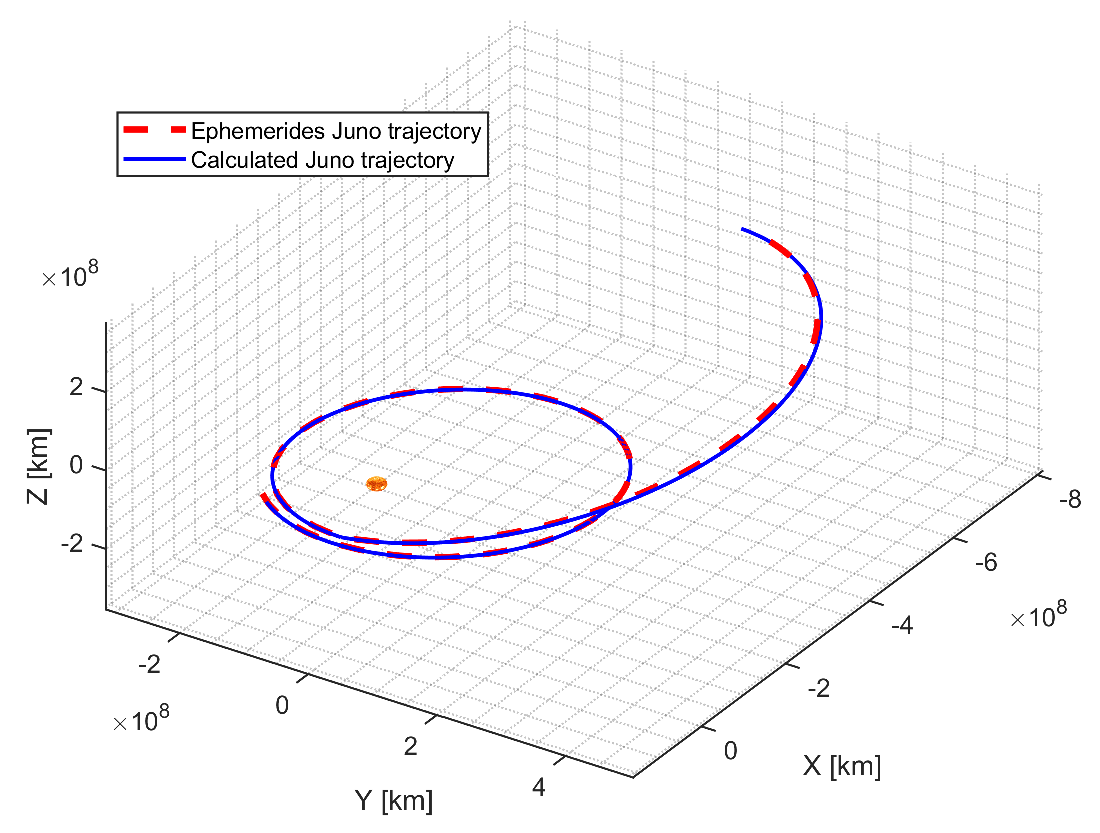
\includegraphics[width=\linewidth]{Images/trajectory.eps}
    \caption{Comparison of trajectories}
    \label{fig:trajectory}
\end{minipage}\hfill
\begin{minipage}{0.5\linewidth}
    \centering
    \captionsetup{type=table}
    \renewcommand{\arraystretch}{1.5}
    \setlength\extrarowheight{-1pt}
    \begin{tabular}{|c|c|c|}
        \hline
        & $\boldsymbol{\Delta V \, [km/s]}$ & $\boldsymbol{Date}$ \\
        \hline
        $\boldsymbol{INJ_E}$ & $5.3920$ & $14/08/2011$ \\
        \hline
        $\boldsymbol{DSM}$ & $0.7225$ & $29/08/2012$ \\
        \hline
        $\boldsymbol{FB}$ & $1.9872 \cdot 10^{-7}$ & $08/10/2013$ \\
        \hline
        $\boldsymbol{INJ_J}$ & $5.4552$ & $09/07/2016$ \\
        \hline
    \end{tabular}
    \caption{Calculated solution}
    \label{table:solution}
\end{minipage} 
The obtained results are coherent with the actual mission data \cite{juno_navigation}. Regarding \autoref{table:solution}, some values might seem particularly high in relation to the main engine capabilities. 
Indeed, not all of the $\Delta V$s had to be performed by the main engine:
\begin{itemize}
    \item $\Delta V_{inj,E}$ was exectued by the upper stage of the Atlas V551, in the limits of the launcher performance $C_3$.
    \item $\Delta V_{inj,J}$ was due to the rendezvous at Jupiter. The only burn required to enter an elliptical orbit had to be given at the pericentre of the hyperbola. The impulsive $\Delta V$ can be calculated as follows, considering $e_{cap} = 0.9884$ and $r_p = $in relation to the designed 107-day orbit: 
    \begin{equation}
        \Delta V_{JOI} = v_{\infty} \left( \sqrt{1 + \frac{2\mu_{J}}{r_p v_{\infty}^2}} - \sqrt{\frac{\mu_{J} (1 + e_{cap})}{r_p v_{\infty}^2}}\right) =  0.km/s 
    \end{equation}
\end{itemize}
Moreover, the low $\Delta V_{fb}$ value in \autoref{table:solution} indicates that gravity assist was not powered. Clean-up maneuver and TCMs were performed before and after the fly-by, hence this small burn.



\cite{fact_sheet}
\begin{table}[H]
    \renewcommand{\arraystretch}{1.3}
    \centering
    \begin{tabular}{|c|c|c|c|c|c|}
        \hline
        \textbf{Manuevers} & \textbf{Design} [m/s] & \textbf{Perf.} [m/s] & \textbf{Sim.} [m/s] & \textbf{$\tau_{ME}$ Design} [min] & \textbf{$\tau_{ME}$ Perf.} [min]  \\
        \hline
        TCM\cite{junno_inner}-$1\div2$ (RCS) & 4.4 & 1.71 & - & - & - \\
        \hline 
        \multicolumn{1}{|c|}{DSM\cite{junno_inner}-1 (ME)} & \multicolumn{1}{c|}{360.1} & \multicolumn{1}{c|}{344.16} & \multirow{2}{*}{722.51} & \multicolumn{1}{c|}{30.97} & \multicolumn{1}{c|}{29.71} \\
        \cline{1-3}
        \cline{5-6}
        \multicolumn{1}{|c|}{DSM\cite{junno_inner}-2 (ME)} & \multicolumn{1}{c|}{394.8} & \multicolumn{1}{c|}{387.94} & & \multicolumn{1}{c|}{30.07} & \multicolumn{1}{c|}{29.77} \\
        \hline
        TCM\cite{junno_inner}-$4\div15$ (RCS) & 32.5 & 7.89 & - & - & - \\
        \hline
        MEF\cite{junno_inner} (ME) & 3.3 & 3.3 & - & - & - \\
        \hline
        JOI\cite{otm} (ME) & $424.07^{\;I}$ & 541.73 & 424.07 & 27.86 & 35.65 \\
        \hline 
        JOI\cite{otm} clean-up (RCS) & 4.92 & 6.39 & - & - & - \\
        \hline
        PRM\cite{otm} (ME) & 636 & - & 602.45 & 35.19 & - \\
        \hline
        OTM\cite{nasa_otm} pre-PC (RCS) & $120^{\;II}$ & 94.88 & - & - & - \\
        \hline 
        PC (RCS) & - & 56.39 & $69.97^{\;III}$ & - & - \\
        \hline
        OTM post-PC (RCS) & - & 108.08 & - & - & - \\
        \hline
        De-Orbit\cite{spaceflight101} (RCS) & $75^{\;IV}$ & $30.89^{\;V} $& 87.93 & - & -\\
        \hline
    \end{tabular}
    \caption{Comparison between estimated and real masses}
    \label{table:masses}
\end{table}

$\;^{I}$ This value has been assumed equal to the one calculated from the insertion on the 107-days orbit. 

$\;^{II}$ This value has been calculated as each of the 30 nominal science orbits require 4 m/s of $\Delta V$.

$\;^{III}$ This value is referred to the plane change of the 53-days orbit as no other trajectories required this manuever. 

$\;^{IV}$ Value assumed to be equal between the 11-days orbit and the 14-days orbit. 

$\;^{V}$ This value has been updated from the nominal 75 m/s since the De-orbit manuever will be performed from a 53-days orbit and not from a 14-days orbit. 

